\documentclass[10pt,a4paper]{article}
\usepackage[margin=2.2cm]{geometry}
\usepackage{fontspec}
\usepackage{kotex}
\setmainfont{Apple SD Gothic Neo}
\setsansfont{Apple SD Gothic Neo}
\usepackage{amsmath,amssymb}
\usepackage{graphicx}
\usepackage{booktabs}
\usepackage{caption}
\usepackage[dvipsnames]{xcolor}
\usepackage[colorlinks=true,linkcolor=MidnightBlue,citecolor=MidnightBlue,
            urlcolor=MidnightBlue]{hyperref}
\usepackage{titlesec}
\titleformat{\section}{\large\bfseries}{\thesection}{0.6em}{}
\titleformat{\subsection}{\normalsize\bfseries}{\thesubsection}{0.5em}{}
\captionsetup{font=small,labelfont=bf}
\setlength{\parskip}{0.35em}
\setlength{\parindent}{0pt}

\usepackage{mdframed}
\newmdenv[linewidth=0.4pt,linecolor=gray!60,backgroundcolor=gray!5,
          innertopmargin=6pt,innerbottommargin=6pt,skipabove=8pt,skipbelow=8pt]{claimbox}
\newcommand{\claim}[2]{\begin{claimbox}\textbf{주장.} #1\par\smallskip
  \textcolor{gray!70}{\textbf{반증 조건.} #2}\end{claimbox}}

\title{\bfseries 스위치는 그 문에 닿지 않았다\\[2pt]
\large 세 번 실패하면 값이 아니라 시점이 죽은 것이다}
\author{월드모델 실험실 · 노트 $796 \sim 797$}
\date{2026-08-07}
\begin{document}\maketitle

\section{한 줄}

논문 $160$ 은 CN 기준선 $0.3094$ 가 \textbf{채택 전 시점}에서 온 값임을 문서로
보였고, 결정적 시험을 등록했다 --- \emph{채택을 되돌리면 노트 $577$ 의 세 값
(KR $0.6374$ · 앱 $0.2897$ · CN $0.3094$)이 나와야 한다.}

\textbf{안 나왔다.} KR 만 $\pm 0.02$ 안이고($+0.0129$), 앱은 $0.1148$ 로
\textbf{채택 전 기록과도} 크게 어긋나며, CN 은 $0.3927$ 이다.

그리고 실패의 모양이 답을 줬다. \textbf{채택 스위치 둘(\texttt{OOC\_DROP} ·
\texttt{orient})을 되돌려도 CN 은 $0.0055$ 밖에 안 움직인다} ---
\texttt{entry\_friction} 이 CN 짝에서 마스크 $0$ 이라 \textbf{스위치가 만질 것이
없다.} 즉 \textbf{CN 격차 $0.0778$ 은 채택 탓이 아니었다.}

씨앗(노트 $793$) · 열(노트 $794$) · 되돌림(노트 $796$) --- 세 시도가 다 실패했다.
노트 $793$ 이 미리 적은 처분을 적용한다: \textbf{CN 을 짝에서 뺀다.}
\textbf{규약 $12$(집 밖 $\geq 2$)는 지금 짝으로 도달 불가 --- 그것이 T$4$ 의
결론이다.}

\begin{figure}[t]\centering
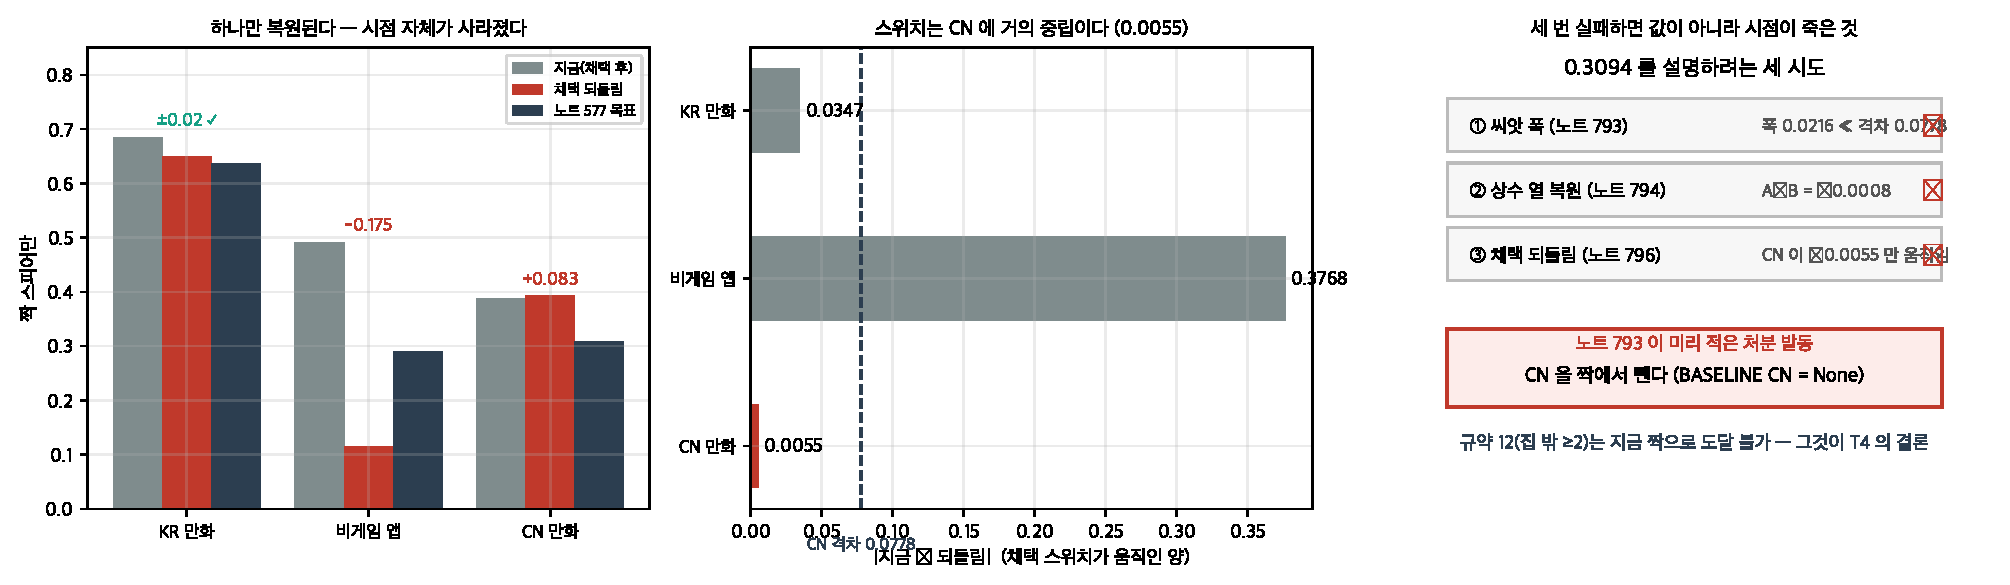
\includegraphics[width=0.99\textwidth]{figs/neutral.pdf}
\caption{왼쪽: 되돌림은 KR 만 복원한다. 가운데: \textbf{스위치가 움직인 양} ---
CN 은 $0.0055$. 오른쪽: 세 시도와 미리 적힌 처분.}
\end{figure}

\section{측정 --- 대조군은 완벽했고 복원은 실패했다}

씨앗 열둘 · 팔 둘(지금 / 되돌림) · 파일은 안 고치고 메모리에서만 되돌렸다
(\texttt{OOC\_DROP = ("entry\_friction",)} 복원 · \texttt{orient} 무력화 ·
커밋 \texttt{bc0b19860} 이 넣은 정확히 그 둘).

\begin{center}
\begin{tabular}{lrrrl}
\toprule
짝 & 지금 & 되돌림 & 노트 $577$ 목표 & $\pm 0.02$ \\
\midrule
KR 만화 & $0.6850$ & $0.6503$ & $0.6374$ & \textbf{✓} ($+0.0129$) \\
비게임 앱 & $0.4916$ & $\mathbf{0.1148}$ & $0.2897$ & ✗ ($-0.1749$) \\
CN 만화 & $0.3872$ & $\mathbf{0.3927}$ & $0.3094$ & ✗ ($+0.0833$) \\
\bottomrule
\end{tabular}
\end{center}

대조군(지금 팔)은 노트 $793$ 을 \textbf{소수 넷째 자리까지} 재현했다(차 $0.0000$
셋 다) --- 배선이 아니라 복원이 실패한 것이다.

\claim{\textbf{노트 $577$ 의 시점은 복원할 수 없다.} 앱이 결정적이다 --- 되돌림이
$0.1148$ 을 내는데 \textbf{채택 전 기록이 $0.2895$ 다.} 스위치 둘 말고도 그
사이에 무엇이(자료 성장 · 파이프라인 변화) 달라졌고, 그것이 무엇인지 이제 알 수
없다. \textbf{규약 $41$ 의 병이 정확히 이 모양이다} --- 재는 코드와 환경이
저장소에 없으면 두 세션 뒤에 그 숫자는 고아가 된다.}
{KR 은 $\pm 0.02$ 안에 들어왔다 --- 복원이 \emph{전혀} 안 되는 것은 아니고
\textbf{짝마다 다르게} 안 된다. 스위치가 앱(\texttt{entry\_friction} 가중
$-0.6353$)에 제일 크게 걸리는 짝이라 다른 변화와의 상호작용도 제일 클 것이다 ---
\textbf{그 상호작용을 안 갈랐다.}}

\subsection*{실패의 모양이 답이다}

\begin{center}
스위치가 움직인 양($|$지금$-$되돌림$|$): KR $0.0347$ · 앱 $\mathbf{0.3768}$ ·
\textbf{CN $0.0055$}
\end{center}

\claim{\textbf{채택 스위치는 CN 에 거의 중립이다.} 둘 다 \texttt{entry\_friction}
을 만지는데 CN 짝에서 그 열은 마스크 $0$ 이다(전부 전연령 · 상수 강등 · 논문
$160$). \textbf{만질 것이 없는 스위치를 아무리 돌려도 문은 안 움직인다.} 따라서
CN 격차 $0.0778$ 은 채택 탓이 아니라 \textbf{노트 $577$ 이후의 재구성 불가능한
드리프트}다 --- 논문 $160$ 의 ``두 시점이 섞인 표''는 문서 사실로 남지만,
\textbf{CN 값 차이의 기제로는 기각된다.}}
{내 사전 예측은 ``(가) 셋 다 맞음''에 $60\%$ 였고 \textbf{틀렸다}(실현된 (다)에
$30\%$). 예측 ② --- \emph{``되돌림 복원이 까다로울 것, 노트 $586$ 이 둘을 함께
바꿨고 어느 쪽이 얼마인지 안 적혀 있다''} --- 는 맞았는데, \textbf{나는 그것을
확률에 제대로 반영하지 않았다.} 까다롭다고 적으면서 $60\%$ 를 걸었다.}

\section{처분 --- 미리 적힌 규칙대로}

노트 $793$ 의 (다): \emph{``$0.3094$ 는 재현 불가 $\to$ CN 을 집 밖 짝에서 뺀다.
그러면 규약 $12$ 는 지금 짝으로 도달 불가이고 그것이 T$4$ 의 결론이 된다.''}

\texttt{lab/pairs.py} 를 고쳤다: \textbf{\texttt{BASELINE} 의 CN 을 \texttt{None}}
으로(규약 $44$ --- 빈 칸은 ``안 쟀다''), 참고값은 \texttt{MEASURED}(씨앗 $12$ ·
SD 포함)로 분리하고 \textbf{시험 ②의 자로는 쓰지 않는다.} 감사표가 지킨다.

\claim{\textbf{규약 $12$ 는 지금 짝으로 도달 불가다.} 만화 열의 집 밖 짝이 KR
하나뿐이고(앱은 모바일 도메인이라 만화 열이 없다) KR 은 $0.0002$ 미달이다(논문
$157$). \textbf{길은 둘뿐이다}: ① KR 짝 행이 \emph{자연히} $1{,}716 \to 1{,}744$
이상으로 자라면 지금 $\Delta$ 로 통과한다(결과를 보고 표본을 늘리는 것은 자를
바꾸는 것이므로 \textbf{기다린다}) ② 만화 도메인의 \textbf{새 집 밖 짝}을 만든다.
어느 쪽도 수집이 먼저다 --- 네 트랙째 같은 결론이다.}
{``도달 불가''는 \textbf{지금 짝} 한정이다. 새 짝 하나(예: 다른 나라 만화 ·
다른 플랫폼)가 서면 바로 뒤집힌다 --- 그리고 그 짝의 기준선은 \textbf{처음부터
씨앗 폭과 시점을 달고} 태어나야 한다(규약 $44$).}

\section{곁가지 --- 오토리서치 하네스 (노트 $797$)}

사용자가 요청했다: \emph{병렬 웹 리서치 · 격리 샌드박스 · 우리 측정 기반 가설 ·
업계 표준 유추 · 검증 · 베스트 채택.} \texttt{serve/research.py} 로 세웠다 ---
여섯 걸음: \textbf{씨앗}(우리 측정에서 출발) $\to$ \textbf{봉인}(가설 + 반증 조건
+ 결정 규칙 세 갈래를 SHA-256 으로) $\to$ \textbf{조사}(가설마다 CLI 서브에이전트
· 빈 임시 디렉터리 · WebSearch/WebFetch/MCP 읽기만 · 병렬 $4$) $\to$
\textbf{대조}(출처 딱지 측정/외부/추정 · \textbf{URL 없는 외부는 코드가 추정으로
강등}) $\to$ \textbf{판정}(봉인된 규칙만) $\to$ \textbf{선발}(기준이 코드에
못박혀 있다 · 후보 없으면 안 고른다). 걸음 사이에 \textbf{훅}이 선다 --- 봉인
모양이 틀리면 게이트가 조사를 막는다.

\claim{\textbf{첫 실전($557$초 · 가설 $3$ 병렬)에서 루프가 ``모르겠다''를 말할 줄
안다는 것을 보였다.} 외부 출처를 $11{\sim}15$개씩 모으고도 판정 나 $1$ · 다 $2$ ·
\textbf{채택 $0$} --- 봉인된 결정 규칙이 요구한 증거 꼴에 못 미쳤기 때문이고,
선발은 억지로 고르지 않았다. 그리고 \textbf{실전이 버그를 하나 찾았다} --- 조사
팔의 MCP 자식 프로세스는 \texttt{warm()} 을 거친 적이 없어 캐시를 두고도 ``판이
안 데워졌다''를 받았다. \texttt{boardsvc.\_ensure()} 로 고쳤다(낼 것들 입구에서
캐시 읽기만 · 적합은 절대 안 건다).}
{한 번 돈 것이다. 봉인 $\to$ 판정의 규칙 준수를 \textbf{모형의 자기 보고}에 상당
부분 의존하고 있고(강등·게이트만 코드다), 판정 프롬프트가 규칙을 실제로 얼마나
지키는지는 \textbf{위약(가짜 증거를 넣은 조사)으로 아직 안 쟀다.}}

\end{document}
